% プラ核講演予稿 geometry版
% 2段組に設定
% 以下を参照して「好ましくない表記」を解消
% % https://ichiro-maruta.blogspot.com/2013/03/latex.html
% 要件は以下の通り(年会HPによる)
% % A4縦,余白各15mm,題目は中央揃えにして1行目から,左上隅に講演番号
% 2018/12/07 T.Yokoyama@The University of Tokyo
\documentclass[a4j,11pt,twocolumn,dvipdfmx,platex]{jarticle}
\usepackage[dvipdfmx]{graphicx,color}
\usepackage[T1]{fontenc}
\usepackage[left=15mm, right=15mm, top=15mm, bottom=15mm]{geometry}

\usepackage{amsmath} %数式環境
\usepackage{bm} %数式中の太字
\usepackage{siunitx} %文章中にSI単位を記述
\usepackage[deluxe]{otf} %フォント管理

\pagestyle{empty} %ページ数を表示しない
\renewcommand{\refname}{References} %参考文献の表示を変更
\renewcommand{\figurename}{Fig.} %Figの表示を変更

% セクション前後の空白を調節
\makeatletter
\renewcommand{\section}{\@startsection {section}{1}{\z@}%
   {.5em \@plus.5em \@minus.2em}%
   {.2em \@plus.3em}%
   {\normalfont\large\bfseries}%
   }
\makeatother


\begin{document}
\twocolumn[
  \noindent
  \begin{flushleft}
      \Large
      \textbf{%%%%%%%%%%%%% この下に講演番号を書いてください。%%%%%
      xPxx
      }
  \end{flushleft}
  \begin{center}
    \Large
    \textrm{%%%%%%%%%%%%% この下にタイトル(和文)を書いてください。%%%%%
    講演予稿サンプル
    }

    \textbf{    %%%%%%%%%%%%% この下にタイトル(英文)を書いてください。%%%%%
    Sample of Abstract
    }

  \vspace{1ex}

  \large \textrm{%%%%%%%%%%%%% この下に著者名(和文)を書いてください。%%%%%
  年会太郎$^1$,核融合次郎2$^2$
  }


  \textrm{%%%%%%%%%%%%% この下に著者名(英文)を書いてください。%%%%%
  Taro Nenkai$^1$, Jiro Kakuyugo$^2$,
  }

  \vspace{1ex}


  \textrm{%%%%%%%%%%%%% この下に所属(和文)を書いてください。%%%%%
  プラズマ大学$^1$,某研究所$^2$
  }

  \textrm{%%%%%%%%%%%%% この下に所属(英文)を書いてください。%%%%%
  Plasma University$^1$, Nanigashi Institute$^2$
  }

  \end{center}
  \normalsize

  \vspace{1ex}
]

%%%%%%%%%%%%% この下に本文を書いてください。%%%%%
\section{本文}
\label{sec:本文}
これはプラズマ核融合学会年会の講演予稿サンプルです.
予稿本文をここに記述します.
A4縦2段組みです.

\begin{figure}[h]
  \centering
  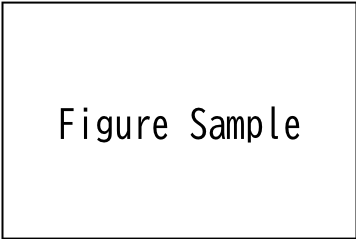
\includegraphics{fig.png}
  \caption{図のサンプル.}
  \label{fig:figure_label}
\end{figure}


%%%%%%%%%%%%% この下に参考文献を書いてください。%%%%%
%\footnotesize
%\bibliographystyle{unsrt_short}
%\bibliography{bibfile}

\end{document}
